\section*{Section A}
\label{sec:Section A}
\FloatBarrier % Now figures cannot float above section title


In this section, the Young's modulus of two materials 
(mild steel and aluminium) can be calculated from experimental data.

A total of six groups of data were obtained from the experiment. (See Table \ref{t1})

\begin{minipage}[t]{\textwidth}
    \makeatletter\def\@captype{table}
    \centering
    \scalebox{1.1}{
    \begin{tabular}{lll} 
        \hline
        No.  & Material    & Final load (N)     \\ \hline
        1 & Steel     & 50    \\
        2 & Steel      & 100   \\
        3 & Steel      & 150   \\
        4 & Aluminium     & 50  \\
        5 & Aluminium    & 100   \\
        6 & Aluminium & 150   \\ \hline          
    \end{tabular}} 
    \caption{result of A1 regression analysis}
    \label{t1} 
\end{minipage}



By plotting these 6 groups of data on a scatter plot and performing 
regression analysis, a total of 6 groups of graphs were obtained.

The results are shown in the next section.


\subsection*{Analysis}





\begin{minipage}[t]{\textwidth}
    \makeatletter\def\@captype{table}
    \centering
    \scalebox{1.1}{
    \begin{tabular}{lll} 
        \hline
        Modulus of Elasticity  & Mild Steel    & Aluminium     \\ \hline
        $E_1(P=50N)$ & 171.482     & 64.3056    \\
        $E_2(P=50N)$ & 175.509     & 64.5370   \\
        $E_3(P=50N)$ & 171.019     & 62.4074   \\
        $E_{exp}=(E_1+E_2+E_3)/3$ & 172.670 & 63.75   \\ \hline          
    \end{tabular}} 
    
    (Unit: GPa)
    \caption{result of A1 regression analysis}
    \label{table4} 
\end{minipage}


\begin{figure}
    \centering
    \includegraphics[]{./fig/1.eps}
    \caption{yes}
    \label{1}
\end{figure}

\subsection*{Summary}